\documentclass{article}
\usepackage{graphicx}
\usepackage{hyperref}
\usepackage{listings}
\usepackage{helvet}
\usepackage{ragged2e}
\usepackage{tikz}
\usepackage{titlesec}
\usepackage{courier}
\usepackage{pdfpages}
\usepackage{xcolor}

%\usepackage{tikz-uml}

\usetikzlibrary{er,positioning, arrows.meta}

\lstset{basicstyle=\footnotesize\ttfamily, language=Java}

\hypersetup{
    colorlinks=true,
    linkcolor=cyan,
    filecolor=magenta,      
    urlcolor=blue,
    pdftitle={Overleaf Example},
    pdfpagemode=FullScreen,
    }
\urlstyle{same}

\definecolor{mygray}{rgb}{0.8,0.8,0.8}
\lstset{
  basicstyle=\ttfamily,
  columns=fullflexible,
  breaklines=true,
  %backgroundcolor=\color{mygray},
  }

\graphicspath{ {./images/} }
%%
%% \BibTeX command to typeset BibTeX logo in the docs
%\AtBeginDocument{%
%  \providecommand\BibTeX{{%
%    Bib\TeX}}}

\titleformat{\section}
  {\normalfont\Large\bfseries}
  {\thesection}
  {1em}
  {}
  [{\titlerule[0.8pt]}]

%\titleformat{\subsection}
%  {\normalfont\Large\bfseries}
%  {\thesection}
%  {1em}
  %{}
  %[{\titlerule[0.3pt]}]

\titleformat{\title}
  {\normalfont\Large\bfseries}
  {\thesection}
  {1em}
  {{\titlerule[0.8pt]}}
  [{\titlerule[0.8pt]}]


\title{
  \line(1,0){250} \\
  \textbf{Multiboxing - A Guide} \\
  v0.9.0 \\
  %%\large \textbf{Final Spec. and Postmortem} \\
  \line(1,0){250}
  }
\author{ 
  Ackbad Pappotte \\\
  }


\renewcommand*\contentsname{Table of Contents}

\begin{document}

%%
%% The "title" command has an optional parameter,
%% allowing the author to define a "short title" to be used in page headers.



\maketitle

\section{Introduction}
Multiboxing is the time honored tradition of creating friends to play with in leu of actually befriending people. This guide aims to be a 
relatively comprehensive look at the process, relevant to running both your 2nd character and your 20th character. This means that you 
should not feel obligated to follow everything outlined in this guide. If you're only running 2 charters for example throttling the FPS of
inactive clients isn't particularly helpful for example. If you find anything incomplete or incorrect, please reach out so I may fix the
issue. Finally, this guide is meant to only cover multi boxing, not alts in general. The latter is far outside of the scope of this guide
and as such is left as an exercise for the reader.

\subsection{Quickstart Checklist}
\begin{enumerate}
  \item Create account via a \href{https://www.eveonline.com/signup?invc=79ffb3de-ef43-400b-a568-e45ac72c6715}{refer a friend link}.
  \item Move to Jita, buy \hyperref[skillplan]{this} skill plan and start it.
  \item Add the new character to your multibox profile in the launcher.
  \item Copy over window layout via the \href{https://github.com/kshannoninnes/CopyEveLayoutTool}{CopyEveLayoutTool}.
  \item Install \href{https://github.com/Proopai/eve-o-preview/releases}{EVE-O Preview}.
  \item \href{https://github.com/Proopai/eve-o-preview}{Configure} EVE-O Preview.
\end{enumerate}

\clearpage
\section{Out of Game Setup}

\subsection{The Rules}
What is not allowed:
\begin{itemize}
  \item Input Broadcasting ie. copping one input across multiple clients. Every input can only correspond to one action
        on a single client (the one exception is if you're using \href{https://wiki.eveuniversity.org/Slash_Commands}{slash command} to 
        queue up commands such as when smartbombing shuttles).
  \item No cutting up the client. You can shrink, resize, and reduce the framerate of a client, but you cannot cut it up.
        \begin{center}
          \makebox[\linewidth]{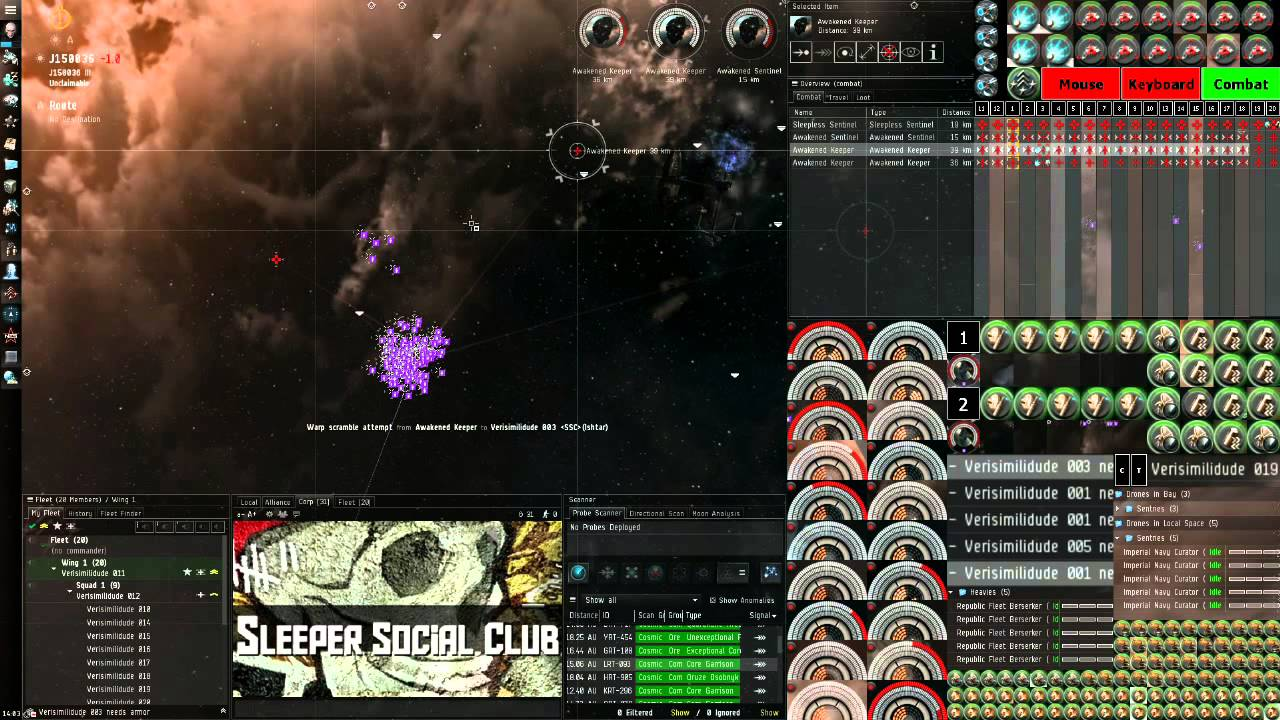
\includegraphics[width=\linewidth]{client_massicure.jpg}}
          An example of a cut up client.
        \end{center}
\end{itemize}
It is worth noting that both of these were once allowed, so particularly old resources and screenshots may reference these now banned techniques.

\subsection{Tools}

\begin{center}
\makebox[\linewidth]{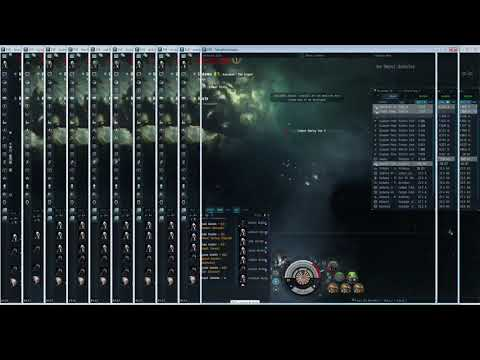
\includegraphics[width=\linewidth]{multiboxing_without_tools.jpeg}}
Multiboxing without a client manager.
\end{center}

\begin{itemize}
  \item \href{https://github.com/Proopai/eve-o-preview}{EVE-O Preview}, Download the latest version \href{https://github.com/Proopai/eve-o-preview/releases}{here} \\
        This is the most popular tool by far because it's both free and build specifically for EVE. It runs on Windows natively, and on Linus
        though Wine. It dose not yet work on Mac.
  \item \href{https://isboxer.com/}{ISBoxer} \\
        This is the main alternative to EVE-O. It is a program that is designed to work across many games, but costs 50\$/year. It
        is generally more powerful letting you configure the resources used by inactive clients, and also allows for banabale techniques
        such as input broadcasting. A guid to setting it up for EVE can be found \href{https://isboxer.com/wiki/EVE:Quick_Start_Guide}{here}.
  \item \href{https://www.guru3d.com/download/rtss-rivatuner-statistics-server-download}{GURU3D RTSS} FPS throttler.\\
        this is a tool to throttle the fps of inactive clients on windows. While windows dose this automatically for minimized clients, if you
        just swap windows it doesn't always happen. This tool also lets you specify the fps of inactive clients. A guide to stetting it up
        for EVE can be found \href{https://www.youtube.com/watch?v=R7YdEPDD_08}{here}.
  \item \href{https://github.com/kshannoninnes/CopyEveLayoutTool}{CopyEveLayoutTool} \\
        \href{https://forums.eveonline.com/t/manually-copy-settings-between-characters-and-accounts/32704}{Instructions to do it manually} \\
        Linux/Steam file location: \lstinline{~/.local/share/Steam/steamapps/compatdata/8500/pfx/drive_c/users/steamuser/AppData/Local/CCP/EVE} \\
\end{itemize}

\clearpage
\subsection{EVE-O Preview Setup}
One of the most important things in multi-boxing is a proper window layout. If you don't want to use eve-o, you can find a good example of how to stack
windows \href{https://www.youtube.com/watch?v=xpiYxq3mpD8}{here}, but this guide assumes you are using eve-o.
\\
recomended settings \\
video of someone using it for 2 clients \\
video of someone using it for 20 clients \\


\clearpage
\subsection{Hotkeys}

If you want to run more then maybe 2 clients you need to setup and learn to use hotkeys as it allows you 
to minimize mouse movement. Particularly if you're running more then 2-3 clients, often you'll be using your
mouse to switch clients so you'll need to use hotkeys so that you don't need to move your mouse across the
screen and back every time you swap to a client to do some input like activating your guns.
\\
\begin{center}
\makebox[\linewidth]{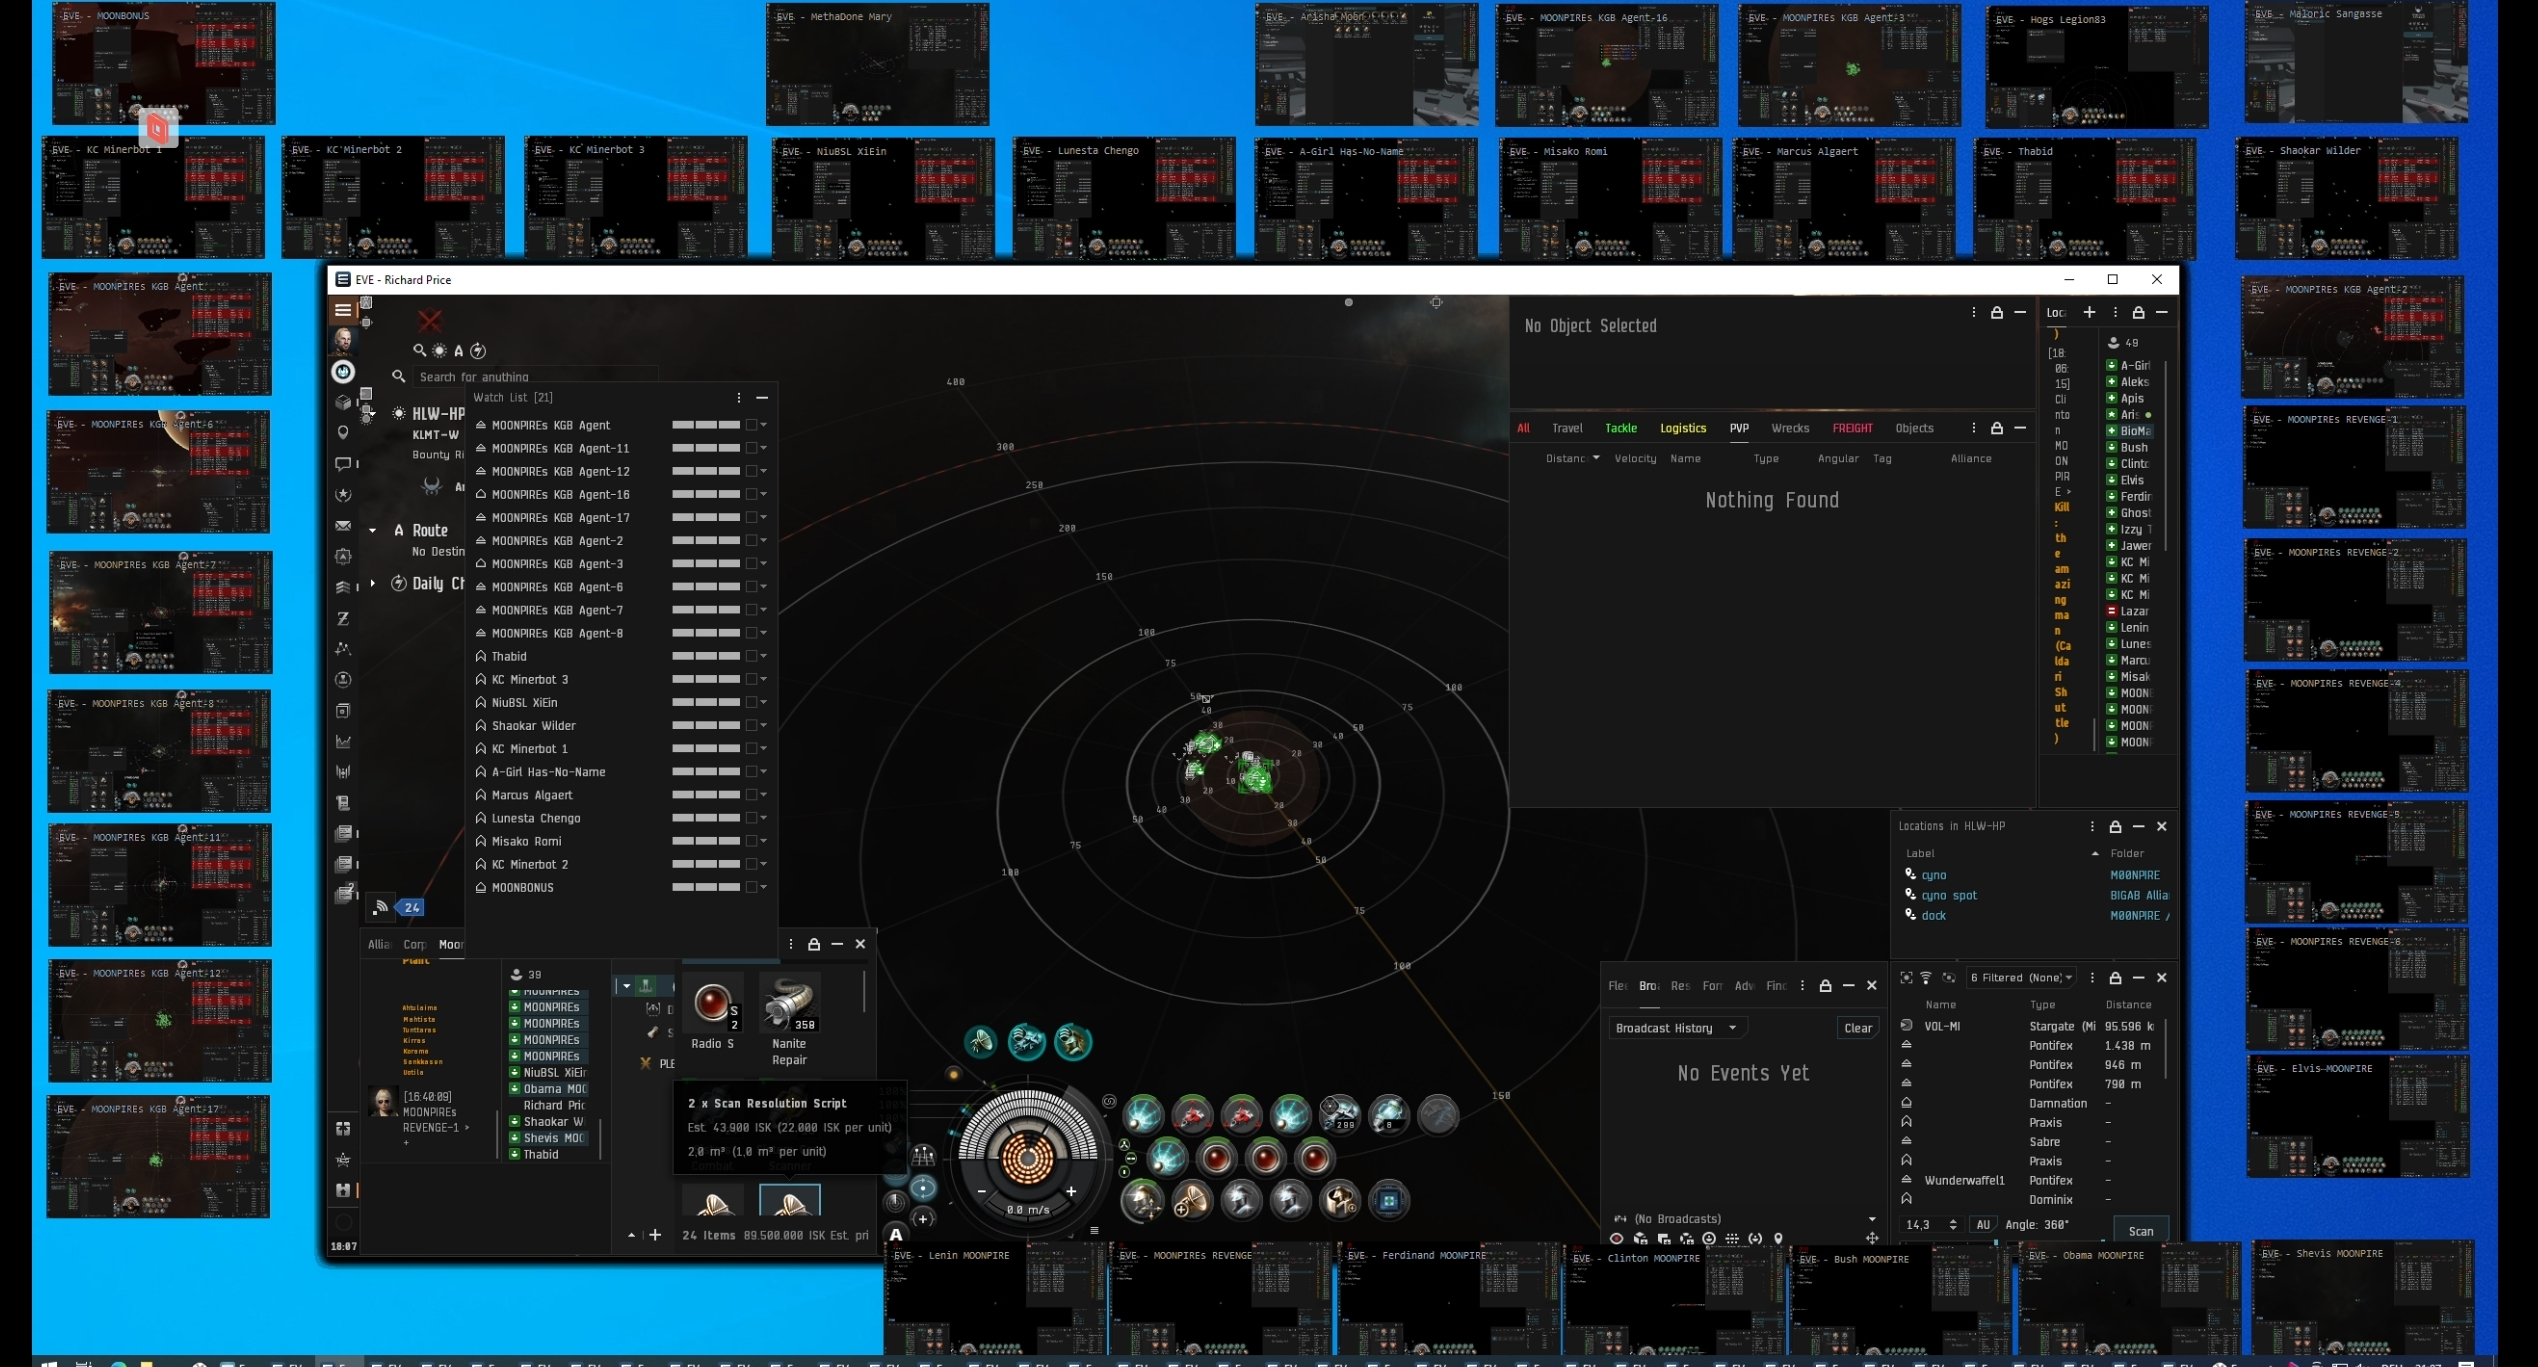
\includegraphics[width=\linewidth]{example_layout.jpg}}
Example layout
\end{center}
While this is an extreem example, you can see how far the mouse would need to move from selecting a client with your mouse,
click a mod, then select the next client. \\

\noindent My setup: \\

\begin{itemize}
  \item 1-0: EVE-O switch client
  \item Q, W, E, R: High-Slots 1-4
  \item A, S, D: Mid-Slots 1-3
  \item Z, X, C: Low-Slots 1-3
  \item F: Lock Target\
  \item V: D-Scan
  \item T: Launch Drones
  \item G: Drones Engage Target
  \item B: Recall Drones to Drone Bay
  \item Y: Broadcast Shield
  \item H: Broadcast Armor
  \item N: Broadcast Capacitor
  \item Mouse Button 4 (Thumb 1): Overheat Modifier Key (shift)
  \item Mouse Button 5 (Thumb 2): Broadcast Target (ctrl)
\end{itemize}

This setup runs into issues with ships like nestors or curses where you can easily have more then 10
 active mods, it is optimized specifically for running 1-3 ships in a nano-gang. The reach to broadcast
 for reps is not ideal either. You don't need to copy this setup, but you should spend some time to
 think out your hotkeys as the defaults are generally terrible.

\clearpage
\subsection{Window Layout}
I'll expand this subsection with example layouts and the logic behind them if there's demand, but tl;dr this guide assumes all eve 
clients are run on a single window, and for this you need a consistent in-game window layout so things like your watchlist location 
and selected item window are in consistent locations as you swap between clients. 
\\


[Add example layout and an explanation]

\clearpage
\subsection{Profiles}
This is a tool built into the EVE client to manage multiple characters at once. It lets you do things like choose a window layout to launch,
with or launch multiple characters simultaneously. 
\\

[Add an actual guide at some point]


\clearpage
\subsection{Tips and Tricks}
\begin{itemize}
  \item A personal chat channel for all your alts. Not only dose this make finding character names for trading and sending isk far easier,
        but the MOTD can also be used to save things like a shared overview that is even accessible if you swap computers.
  \item Bright overview colors. If you want to use the mini client windows provided by EVE-O as eyes, it helps to set all pilots to a default
        bright color so they are more visible in the shrunken down window. Personally I use a solid yellow background for all characters that
        have no standing so neutrals are more easily visible.
  \item When fleet-warping alts around, you can queue up jumping though the gate mid-warp. Just initiate the fleet warp then for every client
        press jump in the selected item window mid-warp and they will all jump on contact with the gate.
\end{itemize}



\clearpage
\section{Character Setup}
\subsection{Character Creation}
To create an account, you'll first need a recruitment link. You can get the recruitment bonus SP retroactively, but you may as well do it now. 
You can generate your own link \href{https://www.eveonline.com/recruit}{here}, or if you can't be bothered you can use \href{https://www.eveonline.com/signup?invc=79ffb3de-ef43-400b-a568-e45ac72c6715}{mine}.
Aside from the bonus SP, whoever generated the link gets minor bonuses if the character created though it buys PLEX or Omega time with cash.
\\
\\
Next, you want to create a Caldari character with any bloodline and the School of Applied Knowledge background. You do this because it spawns
you closest to Jita. Other races may be slightly better in terms of starting skills, but that's at most 10-15m of extra training so I prefer the
closer Jita start.

\clearpage
\subsection{General Skill Plan} 
For early training, I would prioritize 3 things, flying a stiletto, flying a hound, and core skills. The below skill plan will train those 3 things
reasonably well, but skips drone and gun skills. There are many other more specialized roles you may want to train an alt into as well such as links,
logi, ewar, hauling, etc. But an extra tackle/eyes ship and an extra bomber are the two most universally useful and easily trained into. It may also be 
worth re-mapping to optimize this skill plan, but personally I wouldn't recommend any remap beyond dumping Social for the other 4 attributes for such a 
short plan. If you're going to do so though drop the plan in \href{https://evemondevteam.github.io/evemon/}{EVE Mon} to sort the plan by attribute.
Another thing to watch out for is event drugs, as they are often a cheap way to trade sp for isk. They are the reason Biology IV is one of the first 
you train, and they do make Biology V worth it in the long run. Finally, the best way to buy sp for isk is the training boosters in the NES store. While 
slower, they offer a far better isk/sp ratio then skill injectors (particularly after 5m sp) do, though if you plan to go this rout you certainly want to train Biology V.

\label{skillplan}
\begin{lstlisting}
  Science 1
  Science 2
  Science 3
  Cybernetics 1
  Cybernetics 2
  Biology 1
  Biology 2
  Biology 3
  Infomorph Psychology 1
  Infomorph Psychology 2
  Infomorph Psychology 3
  Biology 4
  Spaceship Command 1
  Minmatar Frigate 1
  Minmatar Frigate 2
  Minmatar Frigate 3
  Minmatar Frigate 4
  Minmatar Frigate 5
  Spaceship Command 2
  Spaceship Command 3
  Navigation 1
  Navigation 2
  Evasive Maneuvering 1
  Evasive Maneuvering 2
  Evasive Maneuvering 3
  Evasive Maneuvering 4
  Evasive Maneuvering 5
  Interceptors 1
  Warp Drive Operation 1
  Warp Drive Operation 2
  Warp Drive Operation 3
  Warp Drive Operation 4
  CPU Management 1
  CPU Management 2
  CPU Management 3
  Propulsion Jamming 1
  Propulsion Jamming 2
  Navigation 3
  Afterburner 1
  Afterburner 2
  Afterburner 3
  High Speed Maneuvering 1
  Power Grid Management 1
  Power Grid Management 2
  Shield Upgrades 1
  Mechanics 1
  Hull Upgrades 1
  Hull Upgrades 2
  Hull Upgrades 3
  Hull Upgrades 4
  Spaceship Command 4
  Spaceship Command 5
  Navigation 4
  Interceptors 2
  Interceptors 3
  Interceptors 4
  CPU Management 4
  Power Grid Management 3
  Capacitor Management 1
  Capacitor Management 2
  Capacitor Management 3
  Capacitor Systems Operation 1
  Capacitor Systems Operation 2
  Capacitor Systems Operation 3
  Electronics Upgrades 1
  Electronics Upgrades 2
  Electronics Upgrades 3
  Energy Grid Upgrades 1
  Energy Grid Upgrades 2
  Energy Grid Upgrades 3
  Gunnery 1
  Gunnery 2
  Weapon Upgrades 1
  Weapon Upgrades 2
  Weapon Upgrades 3
  Science 4
  Power Grid Management 4
  Thermodynamics 1
  Thermodynamics 2
  Thermodynamics 3
  High Speed Maneuvering 2
  High Speed Maneuvering 3
  Acceleration Control 1
  Acceleration Control 2
  Acceleration Control 3
  Afterburner 4
  Shield Management 1
  Shield Management 2
  Shield Management 3
  Shield Operation 1
  Shield Operation 2
  Shield Operation 3
  Shield Upgrades 2
  Shield Upgrades 3
  Shield Upgrades 4
  Tactical Shield Manipulation 1
  Tactical Shield Manipulation 2
  Tactical Shield Manipulation 3
  Electronics Upgrades 4
  Electronics Upgrades 5
  Covert Ops 1
  Cloaking 1
  Cloaking 2
  Cloaking 3
  Cloaking 4
  Missile Launcher Operation 1
  Missile Launcher Operation 2
  Light Missiles 1
  Light Missiles 2
  Light Missiles 3
  Missile Launcher Operation 3
  Heavy Missiles 1
  Heavy Missiles 2
  Heavy Missiles 3
  Missile Launcher Operation 4
  Torpedoes 1
  Missile Bombardment 1
  Missile Bombardment 2
  Missile Bombardment 3
  Missile Bombardment 4
  Bomb Deployment 1
  Weapon Upgrades 4
  Missile Launcher Operation 5
  Torpedoes 2
  Torpedoes 3
  Torpedoes 4
  Covert Ops 2
  Covert Ops 3
  Covert Ops 4
  CPU Management 5
  Cynosural Field Theory 1
  Target Navigation Prediction 1
  Target Navigation Prediction 2
  Target Navigation Prediction 3
  Target Navigation Prediction 4
  Warhead Upgrades 1
  Warhead Upgrades 2
  Warhead Upgrades 3
  Warhead Upgrades 4
  Guided Missile Precision 1
  Guided Missile Precision 2
  Guided Missile Precision 3
  Guided Missile Precision 4
  Rapid Launch 1
  Rapid Launch 2
  Rapid Launch 3
  Rapid Launch 4
  Missile Projection 1
  Missile Projection 2
  Missile Projection 3
  Missile Projection 4
  Capacitor Management 4
  Capacitor Systems Operation 4
  Energy Grid Upgrades 4
  Advanced Weapon Upgrades 1
  Advanced Weapon Upgrades 2
  Advanced Weapon Upgrades 3
  Advanced Weapon Upgrades 4
  EM Armor Compensation 1
  EM Armor Compensation 2
  EM Armor Compensation 3
  Explosive Armor Compensation 1
  Explosive Armor Compensation 2
  Explosive Armor Compensation 3
  Thermal Armor Compensation 1
  Thermal Armor Compensation 2
  Thermal Armor Compensation 3
  Kinetic Armor Compensation 1
  Kinetic Armor Compensation 2
  Kinetic Armor Compensation 3
  Mechanics 2
  Mechanics 3
  Mechanics 4
  Mechanics 5
  Hull Upgrades 5
  Armor Layering 1
  Armor Layering 2
  Armor Layering 3
  Armor Layering 4
  Astrometrics 1
  Astrometrics 2
  Astrometrics 3
  Astrometrics 4
  Astrometric Rangefinding 1
  Astrometric Rangefinding 2
  Astrometric Rangefinding 3
  Astrometric Acquisition 1
  Astrometric Acquisition 2
  Astrometric Acquisition 3
  Astrometric Pinpointing 1
  Astrometric Pinpointing 2
  Astrometric Pinpointing 3
  Jury Rigging 1
  Jury Rigging 2
  Jury Rigging 3
  Armor Rigging 1
  Armor Rigging 2
  Armor Rigging 3
  Drones Rigging 1
  Drones Rigging 2
  Drones Rigging 3
  Electronic Superiority Rigging 1
  Electronic Superiority Rigging 2
  Electronic Superiority Rigging 3
  Energy Weapon Rigging 1
  Energy Weapon Rigging 2
  Energy Weapon Rigging 3
  Shield Rigging 1
  Shield Rigging 2
  Shield Rigging 3
  Projectile Weapon Rigging 1
  Projectile Weapon Rigging 2
  Projectile Weapon Rigging 3
  Launcher Rigging 1
  Launcher Rigging 2
  Launcher Rigging 3
  Hybrid Weapon Rigging 1
  Hybrid Weapon Rigging 2
  Hybrid Weapon Rigging 3
  Signature Analysis 1
  Signature Analysis 2
  Signature Analysis 3
  Signature Analysis 4
  Target Management 1
  Target Management 2
  Target Management 3
  Target Management 4
  Long Range Targeting 1
  Long Range Targeting 2
  Long Range Targeting 3
  Long Range Targeting 4
  Gravimetric Sensor Compensation 1
  Gravimetric Sensor Compensation 2
  Gravimetric Sensor Compensation 3
  Ladar Sensor Compensation 1
  Ladar Sensor Compensation 2
  Ladar Sensor Compensation 3
  Radar Sensor Compensation 1
  Radar Sensor Compensation 2
  Radar Sensor Compensation 3
  Magnetometric Sensor Compensation 1
  Magnetometric Sensor Compensation 2
  Magnetometric Sensor Compensation 3
\end{lstlisting}

\clearpage
\subsection{Alpha Training}
If you are planning on training as an alpha, this is the skill plan I would recommend. The main goal is to get you close to flying a hound and stiletto,
with drone and core skills as well as they are so widely applicable. If you are going this rout, do not redeem the 1m sp recruitment bonus to the 
character until after you have finished training, as you can only train to a max of 5m sp on your character sheet, but the bonus sp dose not count
towards this limit until the 1m sp has been redeemed from your redeem queue. Also, if you do not start training immediately you will need to remove
a couple of skills from the end of the queue as it means this plan would put you over 5m sp. The later skills are less important so feel free to drop 
some as necessary. Finally, get a set of +3 implants. They will improve your training time by approximately 30\%, and given that it will take you 5-6 months
to reach 5m sp this is a significant gain for implants that cost ~20m a piece. +4 and +5s are locked behind omega unfortunately. If you get a couple days
of free omega you can inset +5s and retain their benefit while alpha, but free omega is rare enough that this is not worth planning for.

\begin{lstlisting}
Science 1
Science 2
Science 3
Cybernetics 1
Cybernetics 2
Biology 1
Biology 2
Biology 3
Spaceship Command 1
Minmatar Frigate 1
Minmatar Frigate 2
Minmatar Frigate 3
Minmatar Frigate 4
Power Grid Management 1
Power Grid Management 2
Power Grid Management 3
Shield Management 1
Shield Management 2
Shield Management 3
Shield Management 4
Tactical Shield Manipulation 1
Tactical Shield Manipulation 2
Tactical Shield Manipulation 3
Tactical Shield Manipulation 4
Shield Upgrades 1
Shield Upgrades 2
Shield Upgrades 3
Shield Upgrades 4
CPU Management 1
Signature Analysis 1
Signature Analysis 2
Signature Analysis 3
Target Management 1
Target Management 2
Target Management 3
Target Management 4
CPU Management 2
Long Range Targeting 1
Long Range Targeting 2
Long Range Targeting 3
Astrometrics 1
Astrometrics 2
Navigation 1
Navigation 2
Navigation 3
Navigation 4
Warp Drive Operation 1
Warp Drive Operation 2
Warp Drive Operation 3
Afterburner 1
Afterburner 2
Afterburner 3
High Speed Maneuvering 1
High Speed Maneuvering 2
High Speed Maneuvering 3
Evasive Maneuvering 1
Evasive Maneuvering 2
Evasive Maneuvering 3
Acceleration Control 1
Acceleration Control 2
Acceleration Control 3
Afterburner 4
Afterburner 5
Mechanics 1
Mechanics 2
Mechanics 3
Jury Rigging 1
Jury Rigging 2
Jury Rigging 3
Armor Rigging 1
Armor Rigging 2
Armor Rigging 3
Launcher Rigging 1
Launcher Rigging 2
Launcher Rigging 3
Shield Rigging 1
Shield Rigging 2
Shield Rigging 3
Hull Upgrades 1
Hull Upgrades 2
Hull Upgrades 3
Hull Upgrades 4
Hull Upgrades 5
Mechanics 4
Mechanics 5
EM Armor Compensation 1
EM Armor Compensation 2
Explosive Armor Compensation 1
Explosive Armor Compensation 2
Kinetic Armor Compensation 1
Kinetic Armor Compensation 2
Thermal Armor Compensation 1
Thermal Armor Compensation 2
Armor Layering 1
Repair Systems 1
Repair Systems 2
Repair Systems 3
Shield Operation 1
Shield Operation 2
Shield Operation 3
Electronic Warfare 1
Electronic Warfare 2
Electronic Warfare 3
Electronic Warfare 4
CPU Management 3
Propulsion Jamming 1
Propulsion Jamming 2
Propulsion Jamming 3
Propulsion Jamming 4
Target Painting 1
Target Painting 2
Target Painting 3
Sensor Linking 1
Sensor Linking 2
Sensor Linking 3
Weapon Disruption 1
Weapon Disruption 2
Weapon Disruption 3
Missile Launcher Operation 1
Missile Launcher Operation 2
Missile Launcher Operation 3
Missile Launcher Operation 4
Light Missiles 1
Light Missiles 2
Light Missiles 3
Heavy Missiles 1
Heavy Missiles 2
Heavy Missiles 3
Torpedoes 1
Torpedoes 2
Torpedoes 3
Torpedoes 4
Missile Projection 1
Missile Projection 2
Rapid Launch 1
Rapid Launch 2
Rapid Launch 3
Rapid Launch 4
Warhead Upgrades 1
Warhead Upgrades 2
Warhead Upgrades 3
Missile Bombardment 1
Missile Bombardment 2
Missile Bombardment 3
Missile Bombardment 4
Guided Missile Precision 1
Guided Missile Precision 2
Guided Missile Precision 3
CPU Management 4
Capacitor Management 1
Capacitor Management 2
Capacitor Management 3
Capacitor Management 4
Capacitor Management 5
Capacitor Systems Operation 1
Capacitor Systems Operation 2
Capacitor Systems Operation 3
Electronics Upgrades 1
Electronics Upgrades 2
Electronics Upgrades 3
Electronics Upgrades 4
Energy Grid Upgrades 1
Energy Grid Upgrades 2
Energy Grid Upgrades 3
Energy Grid Upgrades 4
Gunnery 1
Gunnery 2
Weapon Upgrades 1
Weapon Upgrades 2
Weapon Upgrades 3
Weapon Upgrades 4
Science 4
Power Grid Management 4
Thermodynamics 1
Thermodynamics 2
Thermodynamics 3
Advanced Weapon Upgrades 1
Advanced Weapon Upgrades 2
Advanced Weapon Upgrades 3
Drones 1
Drones 2
Drones 3
Drones 4
Drones 5
Light Drone Operation 1
Light Drone Operation 2
Light Drone Operation 3
Light Drone Operation 4
Light Drone Operation 5
Amarr Drone Specialization 1
Caldari Drone Specialization 1
Gallente Drone Specialization 1
Gallente Drone Specialization 2
Caldari Drone Specialization 2
Amarr Drone Specialization 2
Minmatar Drone Specialization 1
Minmatar Drone Specialization 2
Drone Avionics 1
Drone Avionics 2
Drone Avionics 3
Drone Avionics 4
Drone Durability 1
Drone Durability 2
Drone Durability 3
Drone Interfacing 1
Drone Interfacing 2
Drone Interfacing 3
Drone Navigation 1
Drone Navigation 2
Drone Navigation 3
Drone Navigation 4
Drone Sharpshooting 1
Drone Sharpshooting 2
Drone Sharpshooting 3
Drone Sharpshooting 4
Medium Drone Operation 1
Medium Drone Operation 2
Medium Drone Operation 3
Heavy Drone Operation 1
Heavy Drone Operation 2
Heavy Drone Operation 3
Gallente Frigate 1
Gallente Frigate 2
Gallente Frigate 3
Gallente Destroyer 1
Gallente Destroyer 2
Gallente Destroyer 3
\end{lstlisting}

\clearpage
\subsection{Skill Farming}
Skill Farming is something you'll need to do if you don't plan on paying for your alt's subscription out of pocket indefinably. While you may want to pay 
for omega initially, eventually you'll run out of skills to train so it becomes worth trading your alt's SP for isk to fund it's subscription. You'll want 
to pick a skill with a long train time, I use Jump Freighters, but Capitol Capacitor Emission Systems is another good option with a shorter training time 
but also fewer requests. You'll want to extract the SP of this skill every month. This can be done remotely so the character dose not need to fly back to 
Jita every month to extract sp. If you want to maximize your skill farming returns you'll need to buy extractors in bulk whenever there is a major sale, 
and by Omega time ideally when there is a big NES sale but if not buy it in 12 month increments. Generally though it is not a good idea to plan on funding
the account purely though skill farming as this also requires you to always sit in a training pod and you need to time the market around unpredictable NES
sales. Instead it is better to treat skill farming as a method of reducing the subscription cost of the account which you can then supplement with other
activities. Ishtar spinning, PI, and mining are all popular options for this, though there are many more avenues you can pursue.



\section*{Appendix A: Links}
\subsection*{Videos}
These are the videos that are linked throughout this guide as well as some that may be helpful but I had no where else to put
\begin{itemize}
  \item \href{https://www.youtube.com/watch?v=dKbQezW0ZwU}{Optomizing for multibox preformance}
  \item \href{https://www.youtube.com/watch?v=Lm4tVwSkBiE}{How to handle information overload}
  \item \href{https://www.youtube.com/watch?v=UpQpgcKSCS4}{EVE-O Preview Video}
  \item \href{https://www.youtube.com/watch?v=xpiYxq3mpD8}{Multiboxing without a client manager}
  \item \href{https://www.youtube.com/watch?v=iC8PwaFf8ck}{Multiboxing 10x marauders}
  \item \href{https://www.youtube.com/watch?v=p5WXd2IkaOc}{Multiboxing 2x nano}
\end{itemize}

\subsection*{Tools}
This is a list of all tools linked throughout this guide.
\begin{itemize}
  \item \href{https://evemondevteam.github.io/evemon/}{EVE Mon}
  \item \href{https://github.com/Proopai/eve-o-preview}{EVE-O Preview}
  \item \href{https://isboxer.com/}{ISBoxer}
  \item \href{https://www.guru3d.com/download/rtss-rivatuner-statistics-server-download}{GURU3D RTSS}
  \item \href{https://github.com/kshannoninnes/CopyEveLayoutTool}{CopyEveLayoutTool}
\end{itemize}

\subsection*{Other Links}
\begin{itemize}
  \item \href{https://forums.eveonline.com/t/manually-copy-settings-between-characters-and-accounts/32704}{Manually coppying window layout}
  \item \href{https://www.eveonline.com/signup?invc=79ffb3de-ef43-400b-a568-e45ac72c6715}{Refer a friend link}
\end{itemize}

\section*{Appendix B: Linux}
\href{https://www.reddit.com/r/Eve/comments/1hqjm4a/linux_lutris_eve_online_eveo_preview/}{Linux Install Guide (Lutris)}\\
As of now there is no known way to run EVE-O and EVE through steam at the same time as proton will only let you run one program 
at a time in a prefix.

% TODO: transcribe the setup guide here, and get the new script link when it's moved to github
% TODO: include bash script to launch EVE-O preview that can be added to the prefix


%\subsection*{EVE-O Install Guide}
%\href{https://www.reddit.com/r/Eve/comments/1hqjm4a/linux_lutris_eve_online_eveo_preview/}{install guide}
%The above link describes the process, but I'll write out the basic process here as well in case it doesn't work.
%\begin{enumerate}
%  \item Install \href{https://lutris.net/}{Lutris}
%  \item Install EVE via the script \href{https://www.reddit.com/r/Eve/comments/1hqjm4a/linux_lutris_eve_online_eveo_preview/}{linked here} or do the following: \\
%    \begin{enumerate}
%      \item Install the Dec. 2023 release of the \href{https://lutris.net/games/eve-online/}{EVE Launcher}
%      \item 
%    \end{enumerate}
%  \item 
%\end{enumerate}

\section*{Appendix C: Mac}
I've never run EVE on a Mac, if you have any insights to share please reach out.

\section*{Appendix D: Skill Plans}
Other skill plans that are useful for alts:

\subsection*{Links}
\subsection*{Cyno}
\subsection*{Hauling}
\subsection*{Logi}
\subsection*{Dred}

\clearpage
\subsection*{Acknowledgments}
Ackbad Pappotte\\
The fine folks of Noir. for catching my many typos.\\
Dal, for helping me troubleshoot EVE-O on the \href{https://discord.gg/xYt8R9AFXB}{discord}. \\
Krombopulous Nathan, for showing up with a lutris install scrip out of nowhere. \\
\\
\\
Want to contribute? Contact Ackbad Pappotte in-game or raise an issue on the \href{https://github.com/AckbadP/eve-multi-guide}{GitHub}.  
\\
%\subsection*{Changelog}



\clearpage
\begin{center}
  \vspace*{\fill}
  %{\Huge \ttfamily O7}\\
  \textsl{\large \ttfamily Fly Dangerous O7}
  \vspace*{\fill}
\end{center}

\end{document}
\endinput